% -*- coding: utf-8; -*-

\chapter{Linha de Mapeamento}

\section{Definição}

Um dos recursos presentes no Sistema Recon é a \textbf{linha de mapeamento}, cujo objetivo é auxiliar na interpretação dos resultados gerados na restauração do modelo. Essa linha armazena referências a pontos topológicos da malha da seção. Com isso, é possível ter uma linha que acompanha a movimentação da malha de um cenário a outro.

As linhas de mapeamento (Figura~\ref{fig-linemap}) permitem realizar um mapeamento geométrico ao longo de uma restauração tomando como base uma linha-guia poligonal definida em um dado cenário. Essa linha pode ser criada em qualquer cenário, mesmo em seções já restauradas.

\begin{figure} [h]
  \begin{center}
    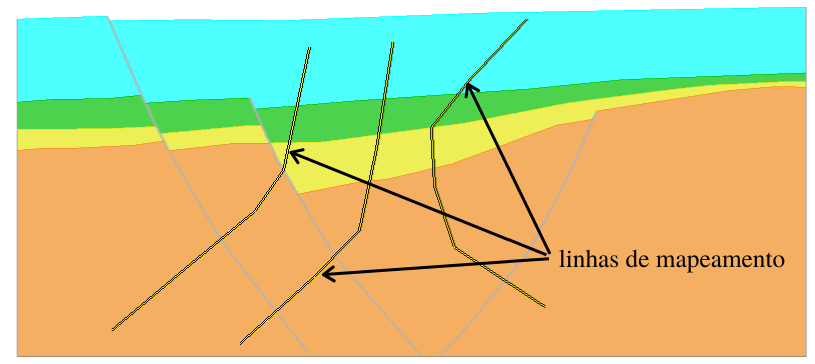
\includegraphics[width=400pt]{images/fig-linhas-de-mapeamento-ed}
    \caption{Linhas de mapeamento em uma seção.}\label{fig-linemap}
  \end{center}
\end{figure}

Cada face de uma seção tem como atributo uma malha triangulada, e as linhas de mapeamento são definidas no sistema de coordenadas local da malha de cada uma das faces. Além disso, é possível que uma linha de mapeamento cruze diversas malhas, por isso, a linha de mapeamento é definida como um conjunto de "partes" de linha de mapeamento, sendo cada parte pertencente a um trecho contínuo em uma mesma face. O processo de criação do mapeamento da linha é feito para cada parte. Na Figura~\ref{fig-linemap-malhas} é possível ver uma linha de mapeamento cortando algumas malhas diferentes.

\begin{figure} [h]
  \begin{center}
    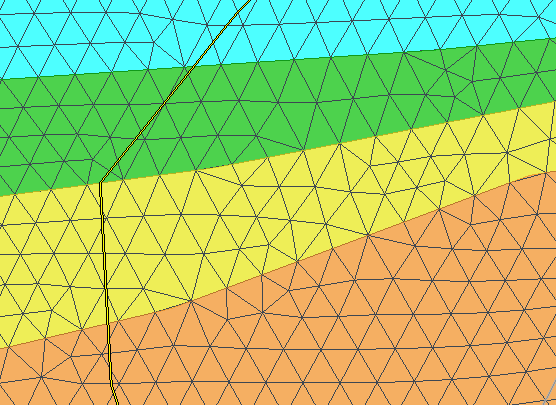
\includegraphics[width=350pt]{images/fig-linhas-de-mapeamento-malhas}
    \caption{Linhas de mapeamento cortando múltiplas faces.}\label{fig-linemap-malhas}
  \end{center}
\end{figure}

A primeira etapa desse mapeamento é a criação da linha-guia, a partir disso é feita a separação nas partes a serem processadas. É realizado um mapeamento com informações topológicas da interseção da parte com a malha. Essa ação consiste em fazer uma relação entre um ponto da parte da linha-guia e um ponto em uma entidade topológica da malha.

Por exemplo, na Figura~\ref{fig-linemap-parts} estão evidenciadas as partes que formam a linha de mapeamento. Cada uma dessas partes é representada pela entidade chamada \textit{LineMapPart}.

\begin{figure} [h]
  \begin{center}
    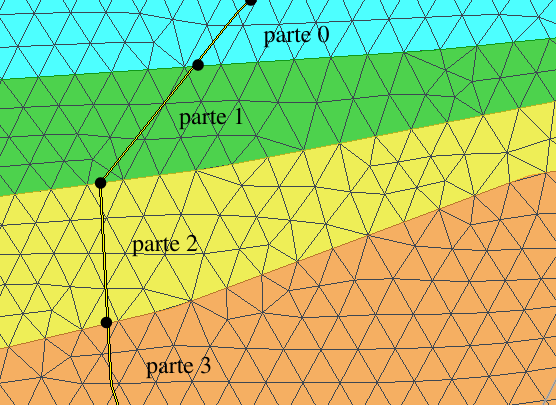
\includegraphics[width=350pt]{images/lm-parts}
    \caption{Partes de uma linha de mapeamento}\label{fig-linemap-parts}
  \end{center}
\end{figure}

Cada parte é processada individualmente e, como já citado, a linha de mapeamento final é um conjunto dessas partes.

Como a malha possui três entidades básicas, o ponto da linha pode ser mapeado para um nó topológico, para um ponto interno de uma aresta (lado de triângulo) de uma malha ou ponto interior a um elemento (triângulo da malha). Em cada um desses casos, a informação topológica relacionada é guardada:

\renewcommand{\labelitemi}{•}
\begin{itemize}
  \item Nó: guarda o indentificador do nó
  \item Aresta: guarda o identificador da aresta e a coordenadas paramétricas do ponto em que cruza a aresta.
  \item Elemento: guarda o identificador do elemento e as coordenadas baricêntricas do ponto no interior do elemento.
\end{itemize}

A Figura~\ref{fig-lm-topo} mostra quais informações topológicas são salvas para uma LineMapPart da linha de mapeamento.

\begin{figure} [h]
  \begin{center}
    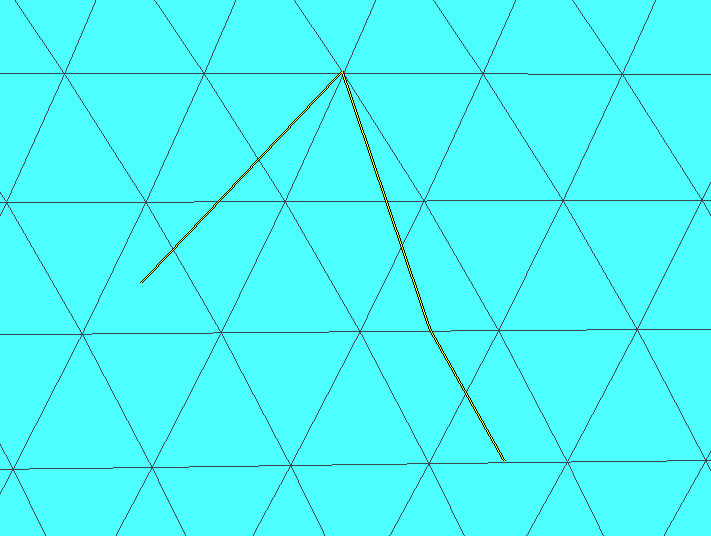
\includegraphics[width=350pt]{images/fig-lm-topo}
    \caption{Informações topológicas da malha mapeadas para a linha de mapeamento.}\label{fig-lm-topo}
  \end{center}
\end{figure}


Após esse processo de mapeamento topológico da linha propriamente dita, é possível calcular a geometria da linha em diferentes cenários que usam a mesma malha (já que a topologia é mantida), bastando apenas verificar se a malha se manteve, isto é, não foi refeita, apagada ou editada.

Em casos de edição, todos os atributos associados à malha são interpolados oara a nova versão da malha, incluem-se nisso as partes de linha de mapeamento que recebem uma nova versão se a malha original teve sua topologia alterada.

A vantagem deste tipo de mapeamento é ser baseado em malha, já que todas as transformações geológicas que ocorrem no processo de restauração, tem como objetivo deformar a malha.

\section{Derivações das Linhas de Mapeamento}

As linhas de mapeamento têm também casos de usos mais especializados, como na criação e representação de poços. Poços são criados semelhantemente às linhas de mapeamento ou por importação de modelos com poços em 3D. Têm característica de serem linhas mais verticalizadas e possuem uma finalidade mais limitada. Nos casos de poços 3D, a linha correspondente ao poço é apenas uma projeção do objeto tridimensional.

Há o uso nas chamadas linhas de interseção (\textit{CrossLine}) que servem para identificar e mapear as linhas de cruzamento entre seções no espaço tridimensional do multi-seções, com isso é possível ter uma noção do que ocorre com seções transversais mesmo estando no domínio bidimensional da restauração.

Por fim, as linhas de mapeamento são a base para a linhas de mapeamento do modelo ou \textit{LMModel}, cujo objetivo é servir como um mapeamento das linhas de entidades geológicas (horizonte, falha e topo de sal) ao longo da restauração do modelo. Dessa forma, é possível ter um acompanhamento das entidades geológicas na seção, baseado na malha das faces que mais bem discretizadas que as arestas base originais, além de poder verificar como se deu a movimentação de cada ponto de horizonte ao longo da restauração, por exemplo.

Pelo objetivo proposto, as LMModels são linhas de mapeamento que tomam a geometria das entidades geológicas como entrada, então não há necessidade de criar uma linha-guia. Neste caso, há uma parte de linha de mapeamento para cada aresta, seja de horizonte, falha ou topo de sal.

Além disso, há o armazenamento de atributos importantes para a manipulação das LMModels, como idade dos horizontes, identificador da falha e até sobre a qual pedaço de superfície aquela parte de linha está associada.

Todas essas informações atreladas ao mapeamento topológico das LMModels, quando em conjunto com as diversas restaurações de um modelo multi-seções, são o que fazem dela o principal dado para a realização de uma restauração a nível 3D, já que trazem todo o histórico de movimentação das camadas de um modelo geológico.
